\documentclass[a4paper,12pt]{article}

\usepackage[utf8]{inputenc}
\usepackage[russian]{babel}
\usepackage[left=17mm, right=15mm, top=20mm, bottom=20mm]{geometry}
\usepackage{pscyr}
\usepackage{moreverb}
\usepackage{graphicx}
    \graphicspath{ {.} }
\usepackage{hyperref}
    \hypersetup{
        colorlinks=true,
        linkcolor=blue,
        filecolor=magenta,      
        urlcolor=cyan,
    }


\begin{document}
    \begin{center}
        \thispagestyle{empty}
        \large САНКТ-ПЕТЕРБУРГСКИЙ ГОСУДАРСТВЕННЫЙ ПОЛИТЕХНИЧЕСКИЙ УНИВЕРСИТЕТ им. ПЕТРА ВЕЛИКОГО

        Институт компьютерных наук и технологий

        Высшая школа искусственного интеллекта
        \vspace{9cm}

        Отчет по курсовой работе

        \huge Игра в дурака
    \end{center}
    \vspace{6cm}
    \begin{flushright}
        \large
        Работу выполнил:

        Алехичев~А.\,В.

        группа~3530201/10001
        \vspace{2mm}

        Проверил:

        Курочкин~Л.\,М.
    \end{flushright}
    \begin{center}
        \large Санкт-Петербург - 2022\,г.
    \end{center}

    \newpage

    \tableofcontents

    \newpage

    \section{Постановка задачи}
        \begin{enumerate}
            \item Разработать алгоритм, который может играть в дурака в качестве игрока по заданным правилам
            \begin{itemize}
                \item Правила находятся в \texttt{/doc/rules.jpg} или по \href{http://13633-oop.mooo.com/files/durak.docx}{ссылке}
            \end{itemize}
			\item Реализовать алгоритм на языке C++, в качестве класса \texttt{Player}.
            \begin{itemize}
                \item Для работы с~колодой использовать статическую библиотеку \texttt{/dealer.lib}.
                \item Сопроводительные файлы к лабораторной и библиотека \textsf{dealer} доступны по~ссылкам: \href{http://13633-oop.mooo.com/files/dealer\_vs2019.zip}{WIN32} или \href{http://13633-oop.mooo.com/files/dealer\_x86\_64.zip}{Linux64}
            \end{itemize}
            \item Подготовить отчёт по~работе, соответствующий требованиям
            \begin{itemize}
                \item Требования находятся в~\texttt{/doc/kr\_req.docx} или по~\href{http://13633-oop.mooo.com/files/kr\_req.docx}{ссылке}
                \item Задокументировать разработанный алгоритм и написанный по~нему код
            \end{itemize}
        \end{enumerate}

    \section{Описание исходных данных задачи}

    \subsection{Алгоритм игры в дурака}
        Данный алгоритм определяет возможные ходы для двух игроков, то как они взаимодействуют и различные состояния игры.
        Алгоритм представлен в~виде блок-схемы, а~также в~файле \texttt{/main.cpp},
        распространяющемся в~одном zip-архиве с~библиотекой dealer.
        Блок-схему можно посмотреть в~\hyperlink{rulesimg}{приложении 1}

    \subsection{Статическая библиотека \textsf{dealer}}
        Дана статическая библиотека \textsf{dealer}.
        Эта библиотека отвечает за контроль колоды и стола.
        К~этому относится: хранение, перетасовка колоды, получение информации о~колоде, взятие карты из~колоды.
        А~также получение информации о~козырной масти и столе.
    
    \section{Определение терминов}
        \subsection{Ранг карты}
            \begin{itemize}
                \item[] Свойство карты.
                \item[] Ранг карты выражается с помощью целого числа --- типа~\texttt{int}.
                \item[] С помощью метода \texttt{Dealer::RankIndex} можно узнать ранг карты.
                \item[] Ранг обычной карты можно использовать как индекс в массиве \texttt{ranks}, чтобы получить имя ранга.
                \item[] Ранг особой карты используется как обозначение состояния особых карт.
                \item[] Данные состояния --- <<Пас>> и <<Без карты>> выражаются числами 300 и 400 соответственно.\\
                        Эти числа указаны в коде как \texttt{PAS} и \texttt{NOCARD}.
                \item[] Ранги обычной карты можно сравнить.
                        Величина ранга увеличивается в порядке:\\
                        \texttt{2 < 3 < 4 < 5 < 6 < 7 < 8 < 9 < 10 < Jack < Queen < King < Ace}.
            \end{itemize}

        \subsection{Масть карты}
            \begin{itemize}
                \item[] Свойство карты.
                \item[] Масть карты выражается с помощью целого числа --- типа~\texttt{int}.
                \item[] С помощью метода \texttt{Dealer::SuitIndex} можно узнать масть карты.
                \item[] Масть обычной карты можно использовать как индекс в массиве \texttt{suits}, чтобы получить имя масти.
                \item[] Масть обычной карты можно использовать как индекс в массиве \texttt{suitsSymb}, чтобы получить символ масти.
                \item[] Масть может быть \textit{козырной}.
                        Масть считается козырной, если совпадает\\с мастью, выбранной дилером до начала игры.\\
                        Эту масть можно узнать с помощью\\метода \texttt{Dealer::GetTrump}.
            \end{itemize}

        \subsection{Карта}
            \begin{itemize}
                \item[] Обычная карта имеет одну из четырёх мастей и один из тринадцати рангов.
                \item[] Особая карта может находиться в одном из двух дополнительных особых состояний: <<Пас>> или <<Без карты>>.
                        В таком случае, её ранг будет равен \texttt{PAS} или \texttt{NOCARD} соответственно.
                \item[] Обычная карта может быть \textit{козырной}.
                        Карта считается козырной, если у неё козырная масть.
                \hypertarget{hit\_rule}{
                \item[] Карта может быть <<атакующей>> или <<защищающей>>.
                        Карта, которой играет игрок с инициативой, называется атакующей.
                        Карта, которой его оппонент может согласно правилам может
                        побить атакующую карту, называется защищающая.
                \item[] <<Атакующую>> карту можно побить <<защищающей>>. Это возможно в одном из двух случаев:
                }
                \begin{itemize} 
                    \item Если карты имеют одинаковую масть, то атакующую карту можно побить защищающей в случае если у первой ранг меньше, чем у второй.
                    \item Если карты имеют разную масть, то атакующую карту любого ранга можно побить козырной защищающей картой любого ранга.
                \end{itemize}
            \end{itemize}

        \subsection{Колода}
            \begin{itemize}
                \item[] Последовательный набор уникальных не особых карт.
                \item[] В начале игры колода из каждой возможной обычной карты перемешивается случайным образом.
                        Таким образом до начала игры в колоде 52 карты.\\
                        За перемешивание колоды отвечает метод \texttt{Dealer::ShuffleDec}
                \item[] Дилер может доставать из колоды карты.
            \end{itemize}

        \subsection{Ход}
            \begin{itemize}
                \item[] Ход это последовательность действий игроков,
                        начинающаяся началом игры или концом другого хода,
                        и заканчивающаяся тем, что игрок без инициативы успешно
                        защитился от атакующих карт или не смог защититься.
                \item[] За ход игрок с инициативой может атаковать шестью картами, в согласии с правилами. 
            \end{itemize}

        \subsection{Стол}
            \begin{itemize}
                \item[] Стол это место, куда игроки разыгрывают карты в соответствии с правилами.
                \item[] На столе лежат карты. Стол имеет тип \texttt{Card*[6]}.
                \item[] За один ход игроки могут сыграть по 6 карт каждый.
            \end{itemize}

        \subsection{Дилер}
            \begin{itemize}
                \item[] Дилер отвечает за управление колодой и столом.
                \item[] Дилер в коде отображён как класс \texttt{Dealer}.
                \item[] Дилер достаёт карты из колоды и раздаёт игрокам в соответствии с правилами игры.\\
                        За это отвечает метод \texttt{Dealer::GetCard}.
                \item[] У дилера можно спросить козырную масть.\\
                        За это отвечает метод \texttt{Dealer::GetTrump}.
                \item[] У дилера можно спросить число вышедших из колоды карт.\\
                        За это отвечает метод \texttt{Dealer::getcurrentCard}.
                \item[] У дилера можно получить указатель на стол.\\
                        За это отвечает метод \texttt{Dealer::GetheadTrick}.
                \item[] У дилера можно узнать номер текущей атакующей карты в ходе.\\
                        За это отвечает метод \texttt{Dealer::GetCurrentHeadTrik}.
                \item[] У дилера можно узнать можно ли сходить атакующей картой.\\
                        За это отвечает метод \texttt{Dealer::NextTrikEnable}.
                \item[] У дилера можно попросить особые карты ''пас'' и ''без карты''.\\
                        За это отвечают методы \texttt{Dealer::GetPas} и \texttt{Dealer::GetNocard}.
                \item[] У дилера можно узнать последнюю атакующую или защищающую карту.\\
                        За это отвечают методы \texttt{Dealer::GetLastCard} и \texttt{Dealer::GetLastDefendCard}.
                \item[] Только с помощью дилера можно атаковать или защищаться картой.\\
                        За это отвечают методы \texttt{Dealer::Attack} и \texttt{Dealer::Defend}.
                \item[] Дилер проверяет защиту от атакующих карт на корректность.\\
                        За это отвечает метод \texttt{Dealer::CheckHeadTrick}.
                \item[] После каждого хода дилер очищает стол от карт.\\
                        За это отвечает метод \texttt{Dealer::ClearTable}.
            \end{itemize}
            
        \subsection{Игрок}
            \begin{itemize}
                \item[] Игрок --- алгоритм или человек, принимающий не противоречащие правилам решения в игре.
                \item[] Один игрок играет лишь за одну сторону.
				\item[] В коде представлен как класс \texttt{Player}, наследующийся от класса \texttt{PlayerAbstract}.
				\item[] Карты игрока, находятся в <<руке>>.
            \end{itemize}
    
    \section{Описание реализации класса Player}
		\subsection {Поля класса Player}
			{\large Определение класса можно найти в \hyperlink{CodePlayerH}{приложении}.}
			\begin{enumerate}
				\item Имя игрока.

					  Так как в функции \texttt{main} в конструктор класса \texttt{Player} зачем-то передаётся имя, то значит надо его хранить.
					  Таким образом, поле на данный момент не выполняет никакой функции.
					  Имя хранится как поле \texttt{const char* m\_name}.

				\item Рука игрока.

					  Рука - массив, где игрок хранит все свои карты.\\
					  Рука хранится как поле \texttt{Card *m\_hand[deckSize]}, где \texttt{deckSize} = 52 --- размер колоды.
					  Указатели на карты могут храниться в руке без определённого порядка, но должны распологаться подряд от нулевого индекса без пробелов.
					  Местам в массиве, которым не назначены указатели на карты, должны быть назначены нулевые указатели.
					  Привести руку к такому состоянию можно с помощью метода \texttt{Player::normalizeHand}.

			  	\item Количество карт в руке.

					  Хранится как поле \texttt{int m\_cardscount}.
				
			    \item Состояние игры.
					
					  Состояние игры - структура с информацией об игре, которую игроку нужно знать.

					  Хранится как поле \texttt{GameState m\_state}.

					  Тип структуры определён как \texttt{struct GameState \{ int trumpSuit; \};}

					  На данный момент структура содержит только поле с текущей козырной мастью --- поле \texttt{trumpSuit}.
					  Это поле хранится тут для удобства.

			\end{enumerate}

		{\large Определения методов класса можно найти в \hyperlink{CodePlayerCPP}{приложении}.}
		
		{\large Блок-схемы, если имеются, находятся в другом документе.}

        \subsection {Метод Player::YouTurn}
			\begin{enumerate}
				\item 	Метод принимает аргумент \texttt{bool flag} --- признак того, что на этом ходу атакует этот игрок.
				\item 	Метод ничего не возвращает.
				\item 	Метод ничего не делает и находится в классе лишь для соответствия интерфейсу класса \texttt{PlayerAbstract}.
			\end{enumerate}

		\subsection {Метод Player::PutCard} % BLOCK
			\begin{enumerate}
				\item 	Метод не принимает аргументов.
				\item 	Метод не возвращает значений.
				\item 	Метод вынуждает игрока атаковать картой (или спасовать).
						По большей части метод выбирает лишь атаковать или нет, а не чем атаковать.
				\item 	Если в руке нет карт, то атаковать нечем, кладём карту <<без карты>>.\\
						Если есть, с помощью метода \texttt{Player::chooseAttackingCard} выбираем карту, которой можно атаковать.\\
						Если на этом ходу мы уже атаковали, то пасуем.\\
						Если нет, атакуем выбранной картой (\texttt{Dealer::Attack}).\\
						Достаём карту из колоды (\texttt{Player::popCard}).
			\end{enumerate}

		\subsection {Метод Player::TakeCards} % BLOCK
			\begin{enumerate}
				\item 	Метод не принимает аргументов.
				\item 	Метод не возвращает значений.
				\item 	Метод берёт все карты со стола.
				\item 	Получаем указатель на стол у дилера (\texttt{Dealer::GetheadTrick}).\\
						В цикле проходим по картам стола.\\
						Если карта --- обычная, то берём её с помощью метода \texttt{Player::TakeOneCard}.
			\end{enumerate}
		\subsection {Метод Player::GetHeadTrick} % BLOCK
			\begin{enumerate}
				\item 	Метод не принимает аргументов.
				\item 	Метод не возвращает значений.
				\item 	Метод вынуждает игрока защититься картой или спасовать.
				\item 	Если последняя атакующая карта была <<пас>> или <<без карты>>, то кладём <<без карты>>.
						Это значит что защищаться не нужно, противник не атакует.\\
						Если не осталось карт в руке, то кладём <<без карты>>.\\
						Принимаем решение, какой картой защищаться (\texttt{Player::chooseDefendingCard}).
						Если метод вернул константу \texttt{unchosen} --- это признак паса.\\
						В остальных случаях метод возвращает индекс карты, которой надо защититься.
						Достаём карту по индексу и защищаемся.
			\end{enumerate}
		\subsection {Метод Player::TakeOneCard}
			\begin{enumerate}
				\item 	Метод принимает аргумент \texttt{Card*\&nc} --- ссылку на карту, которую надо взять в руку.
				\item 	Метод не возвращает значений.
				\item 	Метод помещает карту в руку.
				\item 	В руке в вышеуказанном состоянии, \texttt{m\_cardscount} --- индекс элемента массива, куда надо записать карту.\\
						Записываем туда данный указатель на карту и увеличиваем на 1 значение счётчика \texttt{m\_cardscount}, т.к. карт прибавилось на одну.
			\end{enumerate}
		\subsection {Метод Player::ShowCards}
			\begin{enumerate}
				\item 	Метод не принимает аргументов.
				\item 	Метод не возвращает значений.
				\item 	Метод печатает карты в руке.
				\item 	С помощью цикла проходим по всем картам,
						узнаём их масть и ранг с помощью \texttt{Dealer::SuitName} и \texttt{Dealer::RankName},
						печатаем на экране в формате \texttt{<символ масти><первая буква ранга>} через пробел.

						\textbf{Примечание: ранг 10 печатается как 1.}
			\end{enumerate}
		\subsection {Метод Player::INeedCard}
			\begin{enumerate}
				\item 	Метод не принимает аргументов.
				\item 	Метод возвращает значение типа \texttt{bool} - признак того, что игроку не хватает карт до полной руки.
				\item 	Метод узнаёт, нужны ли карты игроку.
				\item 	Если количество карт в руке $< 6$ и у дилера в колоде остались карты, то возвращает истину. 
			\end{enumerate}
		\subsection {Метод Player::GetCardNum}
			\begin{enumerate}
				\item 	Метод не принимает аргументов.
				\item 	Метод возвращает значение типа \texttt{int} --- количество карт в руке игрока.
				\item   Метод возвращает поле класса \texttt{m\_cardscount}.
			\end{enumerate}
		{\large Дальнейшие методы класса не принадлежат к интерфейсу \texttt{PlayerAbstract}}
		\subsection {Метод Player::normalizeHand}
			\begin{enumerate}
				\item 	Метод не принимает аргументов.
				\item 	Метод не возвращает значений.
				\item 	Метод приводит руку к вышеуказанному виду, сдвигает карты влево по руке.
				\item 	Копируем руку в буфер.\\
						В цикле проходим по буферу, и ставим найденные карты в крайнее левое положение в руку.\\
						Остальную часть руки <<зануляем>> и устанавливаем в счётчик \texttt{m\_cardscount} сколько карт мы нашли.
			\end{enumerate}
		\subsection {Метод Player::less}
			\begin{enumerate}
				\item 	Метод принимает два аргумента -- карты. \texttt{Card* first, Card* secnd}
				\item 	Метод возвращает \texttt{bool} --- признак того, что первая карта <<меньше>> второй.
				\item 	Метод сравнивает две карты.
				\item 	Одна карта <<меньше>> второй, если у первой меньше ранг, или первая уступает в козырности.
			\end{enumerate}
		\subsection {Метод Player::canDefend}
			\begin{enumerate}
				\item 	Метод принимает два аргумента -- карты. \texttt{Card* first, Card* secnd}
				\item 	Метод возвращает \texttt{bool} --- признак того, что первой картой можно побить вторую.
				\item 	Первой картой можно побить вторую, если одно выполняется:
					\begin{enumerate}
						\item 	вторая меньше первой и масти совпадают.
						\item 	вторая уступает в козырности.
					\end{enumerate}
			\end{enumerate}
		\subsection {Метод Player::popCard}
			\begin{enumerate}
				\item  	Метод принимает один аргумент \texttt{int index} --- индекс карты, которую надо достать.
				\item 	Метод возвращает карту, которую надо было достать.
				\item 	Метод достаёт карту из колоды, и поправляет руку.
				\item 	На место нужной карты, ставим \texttt{nullptr}, поправляем колоду и возвращаем карту.
			\end{enumerate}
		\subsection {Метод Player::chooseAttackingCard}
			\begin{enumerate}
				\item 	Метод не принимает аргументов.
				\item 	Метод возвращает индекс (\texttt{int}) карты в руке, которой можно атаковать.
				\item 	Метод выбирает карту, которой можно атаковать, которую меньше всего жалко.
						Сам метод не атакует.
				\item 	В цикле проходим по руке и методом \texttt{Player::less} выбираем <<наименьшую>>.
			\end{enumerate}
		\subsection {Метод Player::chooseDefendingCard} % BLOCK
			\begin{enumerate}
				\item 	Метод не принимает аргументов.
				\item 	Метод возвращает либо индекс (\texttt{int}) карты, которой можно побить атакующую, либо \texttt{unchosen} --- признак паса.
				\item 	Метод выбирает пасовать или защищаться, и если защищаться, то выбирает карту, которой это можно сделать.
				\item 	В цикле выбираем карту наименьшую карту, которой можно защититься от атакующей карты.
				\item 	Если выбрали козырь, то пасуем, возвращая \texttt{unchosen}, если не конец игры.
						В конце игры можно будет использовать козырей.\\
						Возвращаем индекс найденной карты.
			\end{enumerate}
		
	\section{Описание тестирования}
		\begin{itemize}
			\item Класс игрока \texttt{Player} способен играть в соответствии с предоставленными правилами и алгоритмом игры в файле \texttt{main.cpp}.
			\item Библиотека \texttt{VLD} не находит утечек памяти. Это вероятно связано с тем, что я не использую динамически выделенную память.
			\item Тестирование считаю достаточным.
		\end{itemize}
	\section{Заключение}
		\subsection{Изучено} 
			\begin{itemize}
				\item 	В процессе реализации алгоритма я изучил методологию <<Объектно--Ориентированного>> программирования на данном примере.
				\item 	Изучена система вёрстки \LaTeX.
				\item 	Столкнувшись с исключениями возникающими внутри библиотеки, мне пришлось познакомиться с методами реверс-инжиниринга.
						В частности с программами \textsf{gdb}, \textsf{ghidra} и \textsf{objdump}.
						Эти инструменты помогли мне локализовать мою проблему; решить её мне помог исходный код библиотеки.
			\end{itemize}
		\subsection{Освоено} 
			\begin{itemize}
				\item 	Освоена методология ООП, разработка алгоритмов с её помощью.
				\item 	Освоены методы вёрстки документов с помощью \LaTeX.
			\end{itemize}
		\subsection{Реализовано}
			\begin{itemize}
				\item 	Реализован алгоритм игры в дурака по указанным правилам.
						Алгоритм представлен в качестве класса \texttt{Player}.
				\item 	Составлен отчёт в соответствии с требованиями.
				\item 	Программа, симулирующая 100 игр в дурака между копиями реализованного алгоритма.
						Таким образом реализация алгоритма тестируется.
			\end{itemize}
		Всё что реализовано до неопределённого времени доступно в git-репозитории\\
		\href{https://github.com/deutherity/durak}{https://github.com/deutherity/durak}.

    \newpage
    \section{Приложения}
    \hypertarget{rulesimg}{\subsection{Блок-схема алгоритма игры в~дурака (\texttt{/main.cpp})}}
    \begin{figure}[h!]
        \center{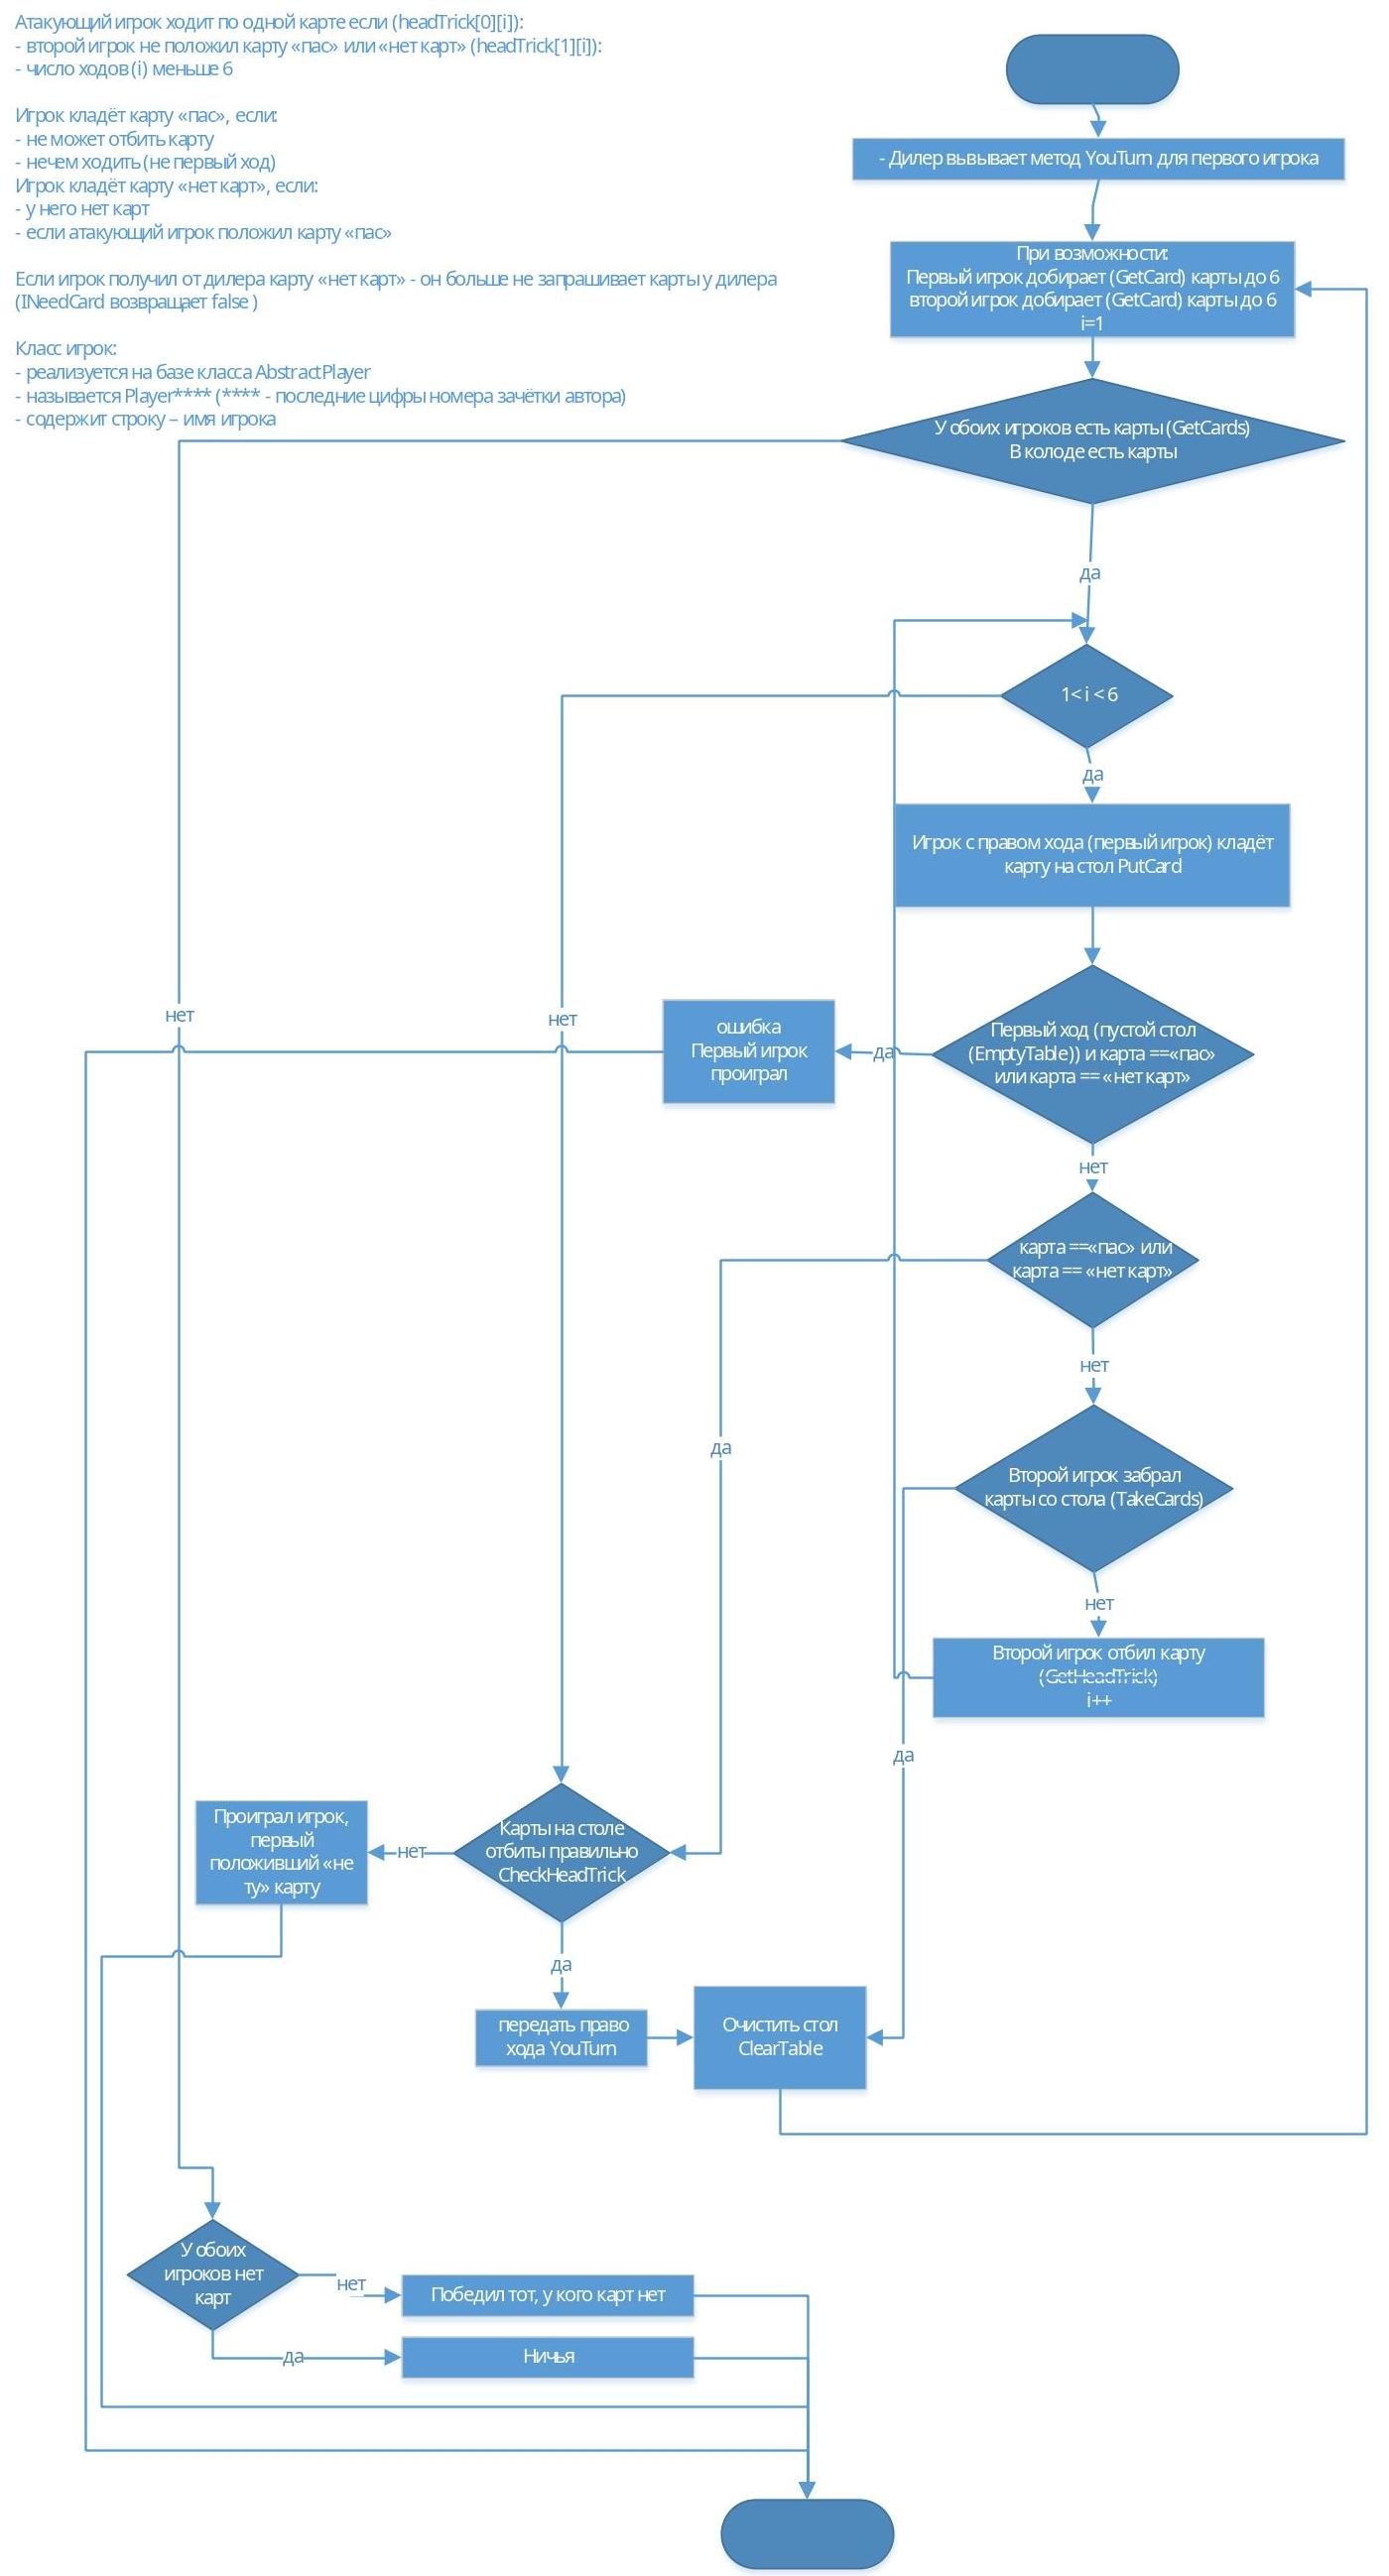
\includegraphics[height=0.9\textheight]{rules.jpg}}
    \end{figure}
    \newpage
	\hypertarget{CodePlayerH}{\subsection{Код файла \texttt{player.h}}}
	\verbatimtabinput[4]{../player.h}
	\hypertarget{CodePlayerCPP}{\subsection{Код файла \texttt{player.cpp}}}
	\verbatimtabinput[4]{../player.cpp}

    %\section{Литература}
    %\newpage
\end{document}
